\chapter{Einführung}
Ziel dieser Vorlesung ist es, die Grundlagen der digitalen Signalverarbeitung (DSV) mit der dazugehörigen Beschreibung durch die Systemtheorie zu
erläutern. Um die Zusammenhänge etwas zu verdeutlichen, gehen wir zunächst der
Frage nach, was ist Nachrichtentechnik, und warum benötigen wir die DSV.

Nachrichtentechnik ist die Lehre von der Übertragung von
Information\footnote{Auf eine formale Definition des Begriffs
Information wird im weiteren Verlauf eingegangen.}. Dabei wird davon ausgegangen, dass es stets eine
Informationsquelle und einen dazugehörigen Empfänger, auch als Senke bezeichnet, gibt.
%
%\begin{figure}[H]
%\begin{center}
%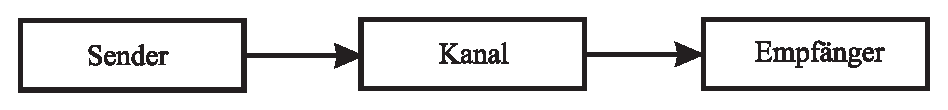
\includegraphics[width = 12cm]{ps/VerallgemeinerteUebertragung.eps}
%\caption{\label{pic:AllgSignalmodell2} Allgemeines Modell für die
%Nachrichtenübertragung.}
%\end{center}
%\end{figure}

\begin{figure}[H]
\begin{center}

\includegraphics[width = 7cm]{ps/AllgSignalmodell}
\caption{\label{pic:AllgSignalmodell} Allgemeines Modell für die
Nachrichtenübertragung.}
\end{center}
\end{figure}


Einige Beispiele für eine solche Übertragung
kennen wir aus unserer täglichen Erfahrung. Wenn wir in einem Gespräch eine
Idee zu unserem Gesprächspartner übertragen wollen, muss zunächst diese Idee in ein
Signal umgewandelt werden, dass über das Medium Luft übertragen werden kann. Beim
Empfänger erfolgt eine hoffentlich fehlerfreie Rückübertragung zum Gehirn.
\begin{figure}[H]
\begin{center}
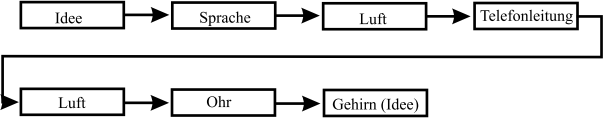
\includegraphics[width = 14cm]{ps/BeispielIdeeIdee}
\caption{\label{pic:BeispielIdeeIdee} Übertragungskette am
Beispiel der Übertragung einer Idee von einer Person zu einer
anderen.}
\end{center}
\end{figure}

Ein weiteres Beispiel ist die Übertragung eines Radioprogramms. Auch hier muss das
eigentlich Nutzssignal zunächst an die Übertragung mittels elektromagnetischer Wellen
angepasst werden.
\begin{figure}[H]
\begin{center}

\includegraphics[width = 7cm]{ps/BeispielRadioLuft}
\caption{\label{pic:BeispielRadio} Übertragungskette am Beispiel
der Rundfunkübertragung.}
\end{center}
\end{figure}

Wir können auch Anwendnungen in unseren Wohnungen finden bei denen sehr komplexe
Übertragungsmechanismen zum Einsatz kommen, \zB das Anhören einer
CD.
\begin{figure}[H]
\begin{center}
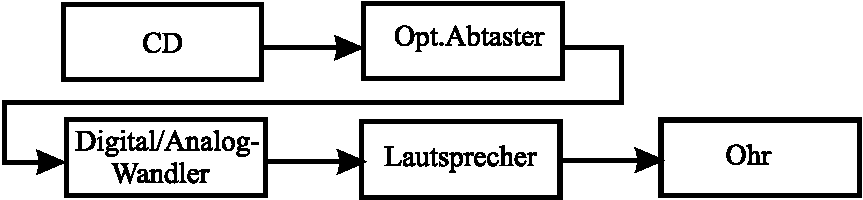
\includegraphics[width = 11cm]{ps/BeispielCDOhr}
\caption{\label{pic:BeispielCDOhr} Übertragungskette am Beispiel
der CD.}
\end{center}
\end{figure}

Aber nicht nur akustische Signale, sondern auch Bilddaten lassen sich in dieses Konzept einpassen,
wie das Beispiel einer Fotoaufnahme zeigt.
\begin{figure}[H]
\begin{center}
\includegraphics[width = 12cm]{ps/BeispielDia}
\caption{\label{pic:BeispielDia} Übertragungskette am Beispiel
eines Landschaftsfotos.}
\end{center}
\end{figure}

Um eine möglichst fehlerfreie Übertragung zu gewährleisten ist es fast immer
notwendig die eigentliche Nachricht zu verändern. Diese
Veränderung kann ganz allgemein als Signalverarbeitung aufgefasst
werde. Da die Signalverarbeitung eine zentrale Aufgabe hat und für
Sie als Studenten von H+A besonders wichtig ist, werden wir uns
zunächst ausschließlich auf die Signalverarbeitung konzentrieren.

\section{Signalverarbeitung}
Die Signalverarbeitung und insbesondere die digitale Signalverarbeitung (DSV) stellt
eine Schlüsseltechnologie für viele moderne Verfahren dar.
Einige Beispiele aus dem Bereich der Telekommunikation und der Sprach- und Audiosignalverarbeitung
sind:
\begin{itemize}
    \item CD-Player
    \item MP3-Player! Gehörbezogene DSV
    \item GSM Mobiltelefon (Handy) (in Zukunft UMTS)
    \item DVD! Visuelle DSV
    \item Synthesizer
\end{itemize}

Das Verständnis der Signalverarbeitung kann insbesondere durch eine einheitliche
Beschreibungssprache erreicht werden, die als Systemtheorie bekannt ist.
Zusätzlich werden nützliche Werkzeuge bereitgestellt, die
eine umfangreiche und in vielen Fällen vollständige
Analyse der Signalverarbeitungsalgorithmen ermöglichen.

\section{Systemtheorie}
Die Systemtheorie ist ein sehr mächtiges Werkzeug zur Beschreibung von SV-Algorithmen.
Gleichzeitig wird die Systemtheorie auch in anderen technischen Bereichen eingesetzt, \zB
in der Automatisierungstechnik. Um die Zusammenhänge etwas zu verdeutlichen, zeigt
Abbildung \ref{pic:SystemtheorieEinordnung} wie die einzelnen Themengebiete
miteinander in Verbindung stehen. Die Systemtheorie ist dabei von so elementarer Bedeutung,
dass zunächst einige Grundbegriffe der Systemtheorie behandelt werden, wie sie für die DSV
benötigt werden.

\begin{figure}[H]
\begin{center}
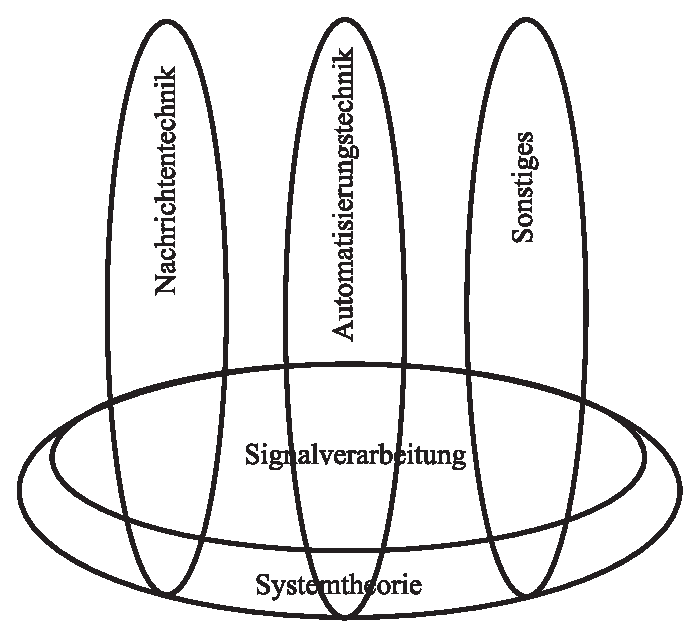
\includegraphics[width = 6cm]{ps/SystemtheorieEinordnung}
\caption{\label{pic:SystemtheorieEinordnung} Zur Einordnung der Systemtheorie.}
\end{center}
\end{figure}
